In the seminal paper by Einstein \cite{einsteinUberErzeugungUnd1905}, that laid foundations to Quantum Mechanics, Einstein postulated that light is made of discrete quanta of energy $E = h\nu$ to explain the observations by Hertz and J.J. Thompson; explaining the photoelectric effect. The effect can be described by the Equation \ref{eq:photoelectric} where $E_e$ the emitted kinetic energy, $h$ is the plank's constant, $\nu$ the frequency of the incoming photon and  $\phi$ the material-specific work function (also known as binding energy). 

\begin{equation}\label{eq:photoelectric}
    E_e = h\nu - \phi
\end{equation}

The equation describes how incident photons on a surface eject photoelectrons, provided the photon energy $h\nu$ exceeds $\phi$. This also highlights that the emitted kinetic energy $E_e$ does not depend on the photon flux (photon counts per second). However, the flux increases the total amount of electrons released from the material.

It is then apparent that the binding energy of electrons can be found by irradiating light onto the material and measuring the $E_e$ of photoelectrons. \gls{PES}, is exactly such a technique that leverages this principle to probe the electronic structure of materials. While the above equation describes at what energies electron come out, it does not explain why 



A complete treatment of photoemission process needs the quantum theory of light-matter interaction, and this shall be introduced where necessary. 

\section{Light-Matter Interaction}\label{section:light-matter-interaction}
Where a complete description is not always necessary.

\section{Light Sources}\label{section:light-sources}
Table top, Synchrotrons, FELs. Time resolved PES and how it relates to acquisition times.


\section{SASE FELs}
\gls*{DESY} is a national 

\begin{figure}
    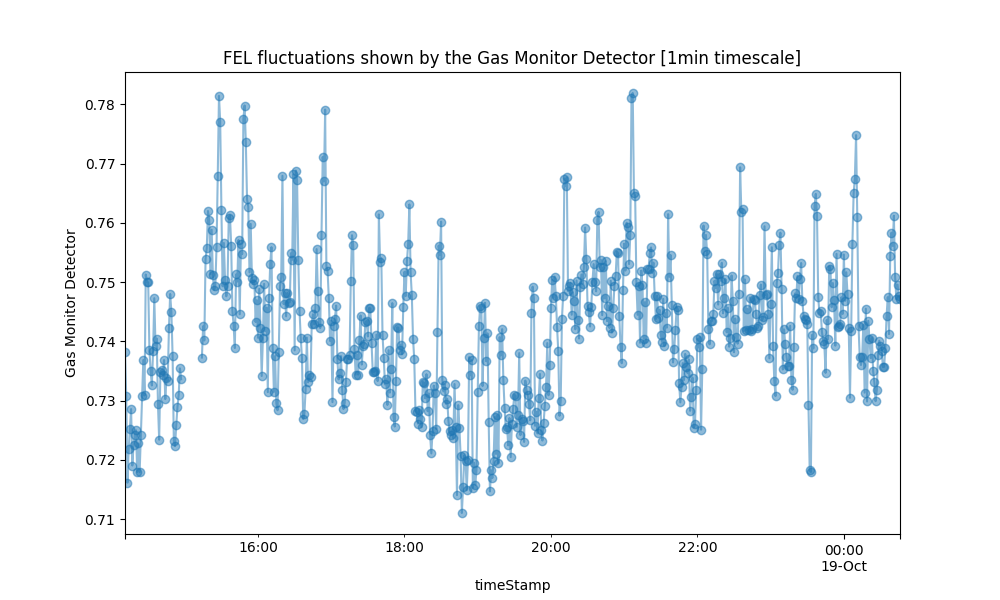
\includegraphics[width=1\linewidth]{images/2024-08-16-13-56-32.png}
\end{figure}



\section{HEXTOF instrument at FLASH}
A variety of photoemission spectrometers can be devised depending on which parameters are varied and what is measured. Naturally, the most basic setup would measure the energy of the emitted electron as described in equation \ref{eq:photoelectric}, but it is also common to measure the surface parallel momentum ($k_x$, $k_y$)

the whole process of excitation, transport, and emission is treated as a single coherent process using the formalism of quantum mechanics. This approach incorporates the electronic structure, electron-electron interactions, and the surface barrier in a unified way, and describes the photoemission intensity  I(E, $k_x$, $k_y$)  as:

% I(E, k_x, k_y) \propto |\langle \psi_f | \mathbf{A} \cdot \mathbf{p} | \psi_i \rangle|^2 \delta(E - E_f)

% where:

% 	•	 \psi_i  and  \psi_f  are the initial and final electron wavefunctions.
% 	•	 \mathbf{A} \cdot \mathbf{p}  is the interaction term representing the coupling between the electron and the incident photon (with vector potential  \mathbf{A}  and momentum operator  \mathbf{p} ).
% 	•	The delta function  \delta(E - E_f)  ensures energy conservation.


The \gls{HEXTOF} instrument is capable of performing time- and momentum-resolved photoemission studies 
\begin{figure}
    \centering
    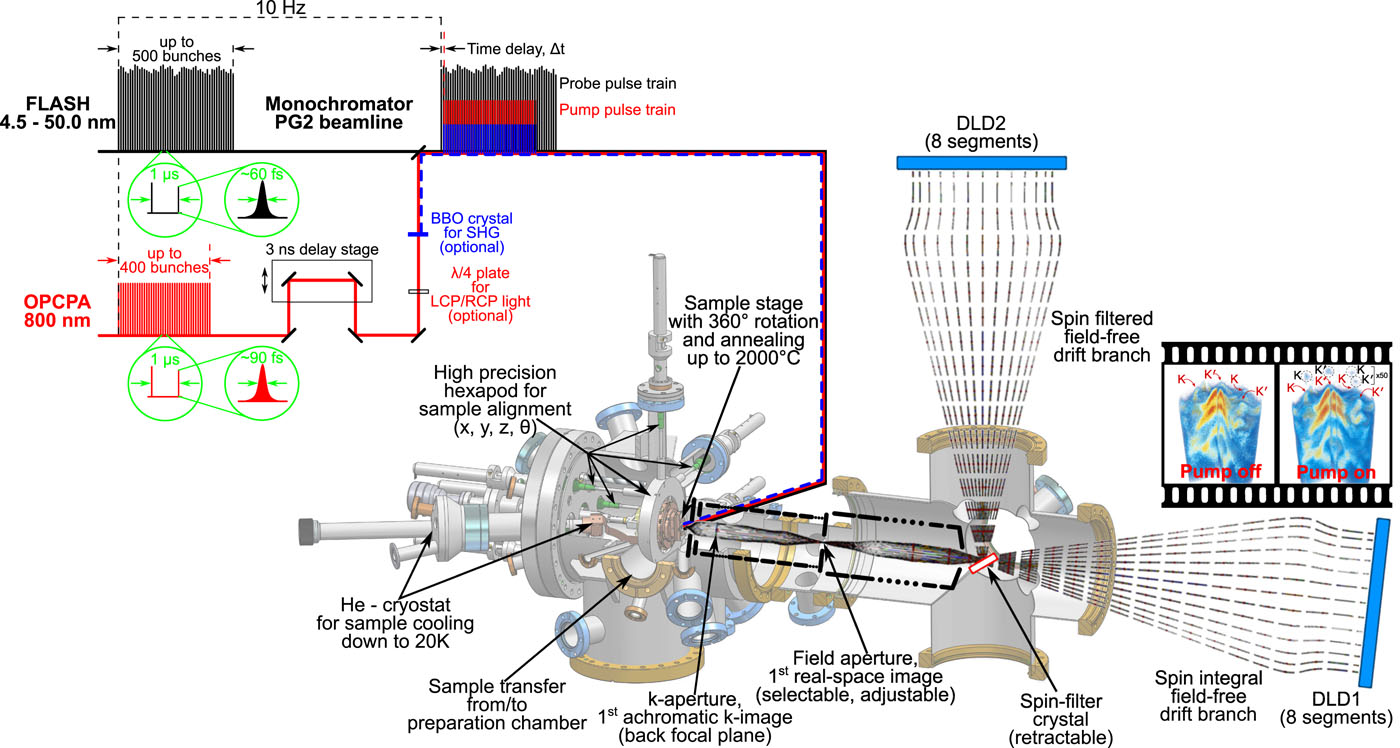
\includegraphics[width=1\linewidth]{images/2024-08-27-10-50-01.png}
    \caption{HEXTOF taken from \cite{kutnyakhovTimeMomentumresolvedPhotoemission2020}}
    % \label{fig:enter-label}
\end{figure}

\subsection{Delay Line Detectors}
The 3D detection scheme used in the \gls{HEXTOF} instrument consists of a \gls{DLD} and a \gls{TOF} tube. The \gls{DLD} is made of a \gls{MCP} for electron amplification and meanders to 

A Delayline Detector (DLD) operates by using a serpentine wire arrangement (meanders) positioned behind a micro-channel plate (MCP) for electron amplification. When particles (photons, ions, electrons) hit the MCP, they generate an electron cloud that induces electrical pulses in the meanders, allowing for precise time measurement of the hit position. This enables the reconstruction of the impact location and provides absolute time measurements relative to an external clock signal, processed by fast electronics and a time-to-digital converter (TDC).

\begin{figure}
    \centering
    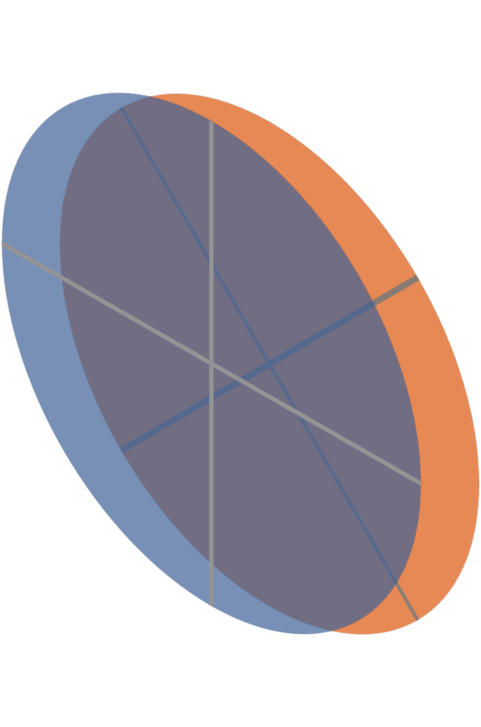
\includegraphics[width=0.3\linewidth]{images/sectors_figure.pdf}
    \caption{Schematic of the 2-layered DLD. The detector is divided into 2 layers, each with 4 sectors.}
    \label{fig:sectors}
\end{figure}

%images/chessy_deblurring_merged_events.png
\begin{figure}
    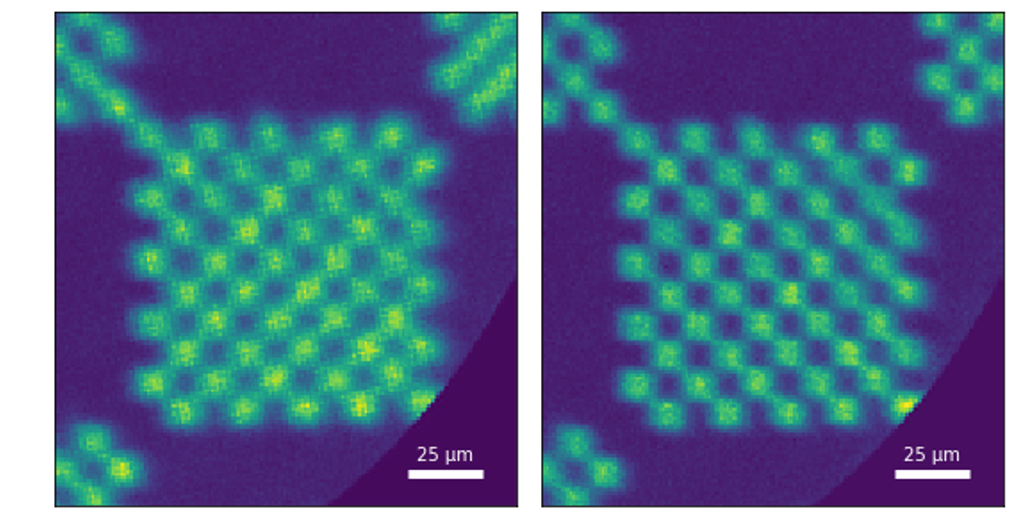
\includegraphics[width=1\linewidth]{images/chessy_deblurring_merged_events.png}
\end{figure}

\section{Binning as means of Imaging}
digital imaging from lecture
sampling etc
Binning is a way to find underlying distribution.


\section{Describing the data GdW, WSe2, GrIr, and new one}

\section{Creating the dataset Corrections Calibrations etc}
\begin{figure}
    \centering
    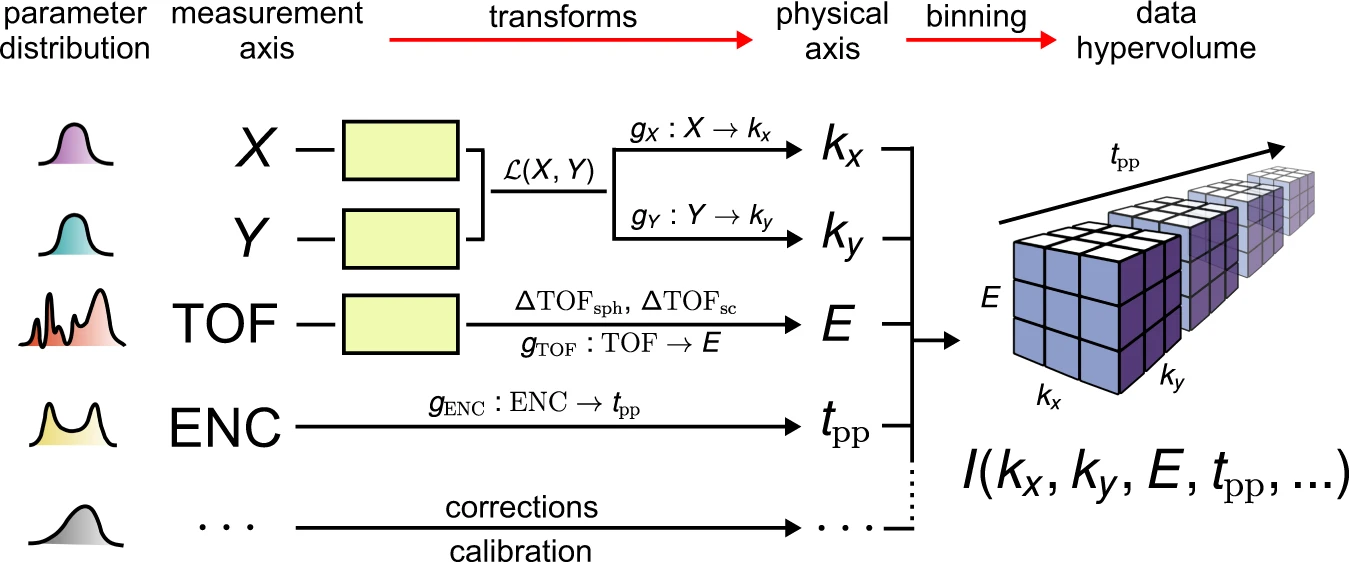
\includegraphics[width=1\linewidth]{images/2024-08-25-22-36-44.png}
    \caption{MPES taken from \cite{xianOpensourceEndtoendWorkflow2020}}
    % \label{fig:enter-label}
\end{figure}